\documentclass[main.tex]{subfiles}
\begin{document}

\section{Parsing and Classification}
\setcounter{section}{4}
%\setcounter{table}{0}
%\setcounter{figure}{0}
\subsection{Choice of Language}

With very few exceptions, the code written in support of this thesis was done in Clojure, a dialect of LISP designed to work on top of the Java Virtual Machine (JVM). The choice of language was simple: a heavy dependence on the Stanford Parser and the Weka package, both written in Java, necessitated a JVM-based language. The slowness of Java's compile/debug cycle eliminated that language as an option, leaving a handful of possible languages, from which Clojure was chosen for its speed, functional style, and elegance.

\subsection{Parsing}
\label{subsec:parsing}

The Stanford Parser software package, version 1.6.7, configured with the included probabilistic context-free grammar (PCFG) \citep*{klein-manning-pcfg:2003}, was used to generate all syntactic parse trees and grammar dependency graphs. A detailed description of PCFGs is beyond the scope of this paper, and the reader who desires such is referred to \citet{booth:1973}. Central to the PCFG is the context-free grammar (or \textit{phrase structure grammar}). A context-free grammar consists of a number of rules, each of which describe the various possible compositions of a particular type of phrase. For instance, Figure~\ref{fig:ps-rules} shows a very simple English grammar consisting of five rules.
\begin{figure}
\centering
\begin{tabular}{l l l l}
a. & S & $\rightarrow$ & $\text{NP} \text{ VP}$\\ 
b. & NP & $\rightarrow$ & $(\text{Det}) \text{ N } (\text{PP})$\\
c. & VP & $\rightarrow$ & $(\text{Aux}) \text{ V } (\text{NP}) \text{ } (\text{AdvP})^n$\\
d. & PP & $\rightarrow$ & $\text{P } \text{NP}$\\
e. & AdvP &  $\rightarrow$ & $\begin{Bmatrix}
\text{Adv} \\ \text{PP} \\
\end{Bmatrix} $
\end{tabular}
\captiont{Simple Phrase Structure Rules}{\citep[p. 195]{akmajian:2010}}
\label{fig:ps-rules}
\end{figure}
Rule (a) indicates that a sentence (S) is composed of a noun phrase (NP) followed by a verb phrase (VP). Rule (b) says that a noun phrase is composed of a noun (N) preceded by an optional determiner (Det), and followed by an optional prepositional phrase (PP). Rule (c) says that a verb phrase contains an optional auxiliary verb (Aux), followed by a verb (V), followed by an optional noun phrase, and then by zero or more adverbial phrases (AdvP). A prepositional phrase is defined by rule (d) as being a preposition plus a noun phrase, and an adverbial phrase is defined by rule (e) as being either an adverb or a prepositional phrase. Again, these are only example rules and cover just a small subset of English grammar. Also, the symbols used by the Stanford parser are not necessarily the same used in these example rules. Using these rules, the sentence \textit{the sun will dry the grapes} can be represented as the tree shown in Figure~\ref{fig:ps-tree}.
\begin{figure}[htbp]
\centering
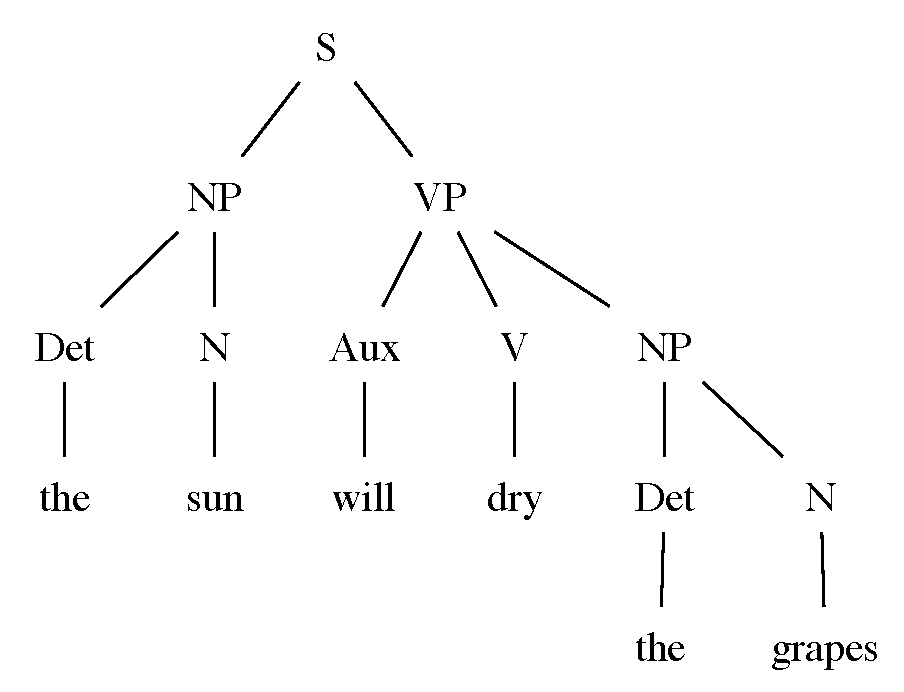
\includegraphics[scale=0.6]{ps-tree.pdf}
\caption[Parse of \textit{the sun will dry the grapes}]{Parse of \textit{the sun will dry the grapes}, Generated from Rules in Figure~\ref{fig:ps-rules}}
\label{fig:ps-tree}
\end{figure}
Generating this tree from the original sentence requires a certain knowledge of the parts of speech of the words in the sentence. To some extent, it is not necessary to have all of this information. In fact, if any of the open-class\footnote{\textit{Open-class words} are those belonging to a class which allows the admission of new words, such as nouns and verbs. \textit{Closed-class words} belong to class which do not generally admit new entries, such as prepositions and articles. Open-class words are often called \textit{content} words and closed-class words \textit{function} words. In this example \textit{sun}, \textit{dry}, and \textit{grapes} belong to open-classes and \textit{the} and \textit{will} to closed-classes.} words in this example are replaced with nonsense words, most people would have no trouble parsing it, and would generate a tree with the same structure as that in Figure~\ref{fig:ps-tree}. Similarly, the Stanford parser successfully parses this sentence even if all of the open-class words are replaced with nonsense words. This does not always hold true for more complex sentences. Also, replacing the closed-class words with gibberish makes the sentence much more difficult to parse, as does replacing one word with another word of a different part of speech (e.g. \textit{the sun will dry the warmly}). Parsers guess the part of speech of unknown words the same way humans do, by choosing whatever part of speech produces the most common valid phrase structure. Parsers use a similar method for dealing with ambiguities.

Consider the sentence \textit{the bag was found in the woods by a farmer}. Using the phrase structure rules from Figure~\ref{fig:ps-rules}, one could generate either the parse shown in Figure~\ref{fig:ps-tree-ambig1} or that shown in Figure~\ref{fig:ps-tree-ambig2}. 
\begin{figure}[htbp]
\centering
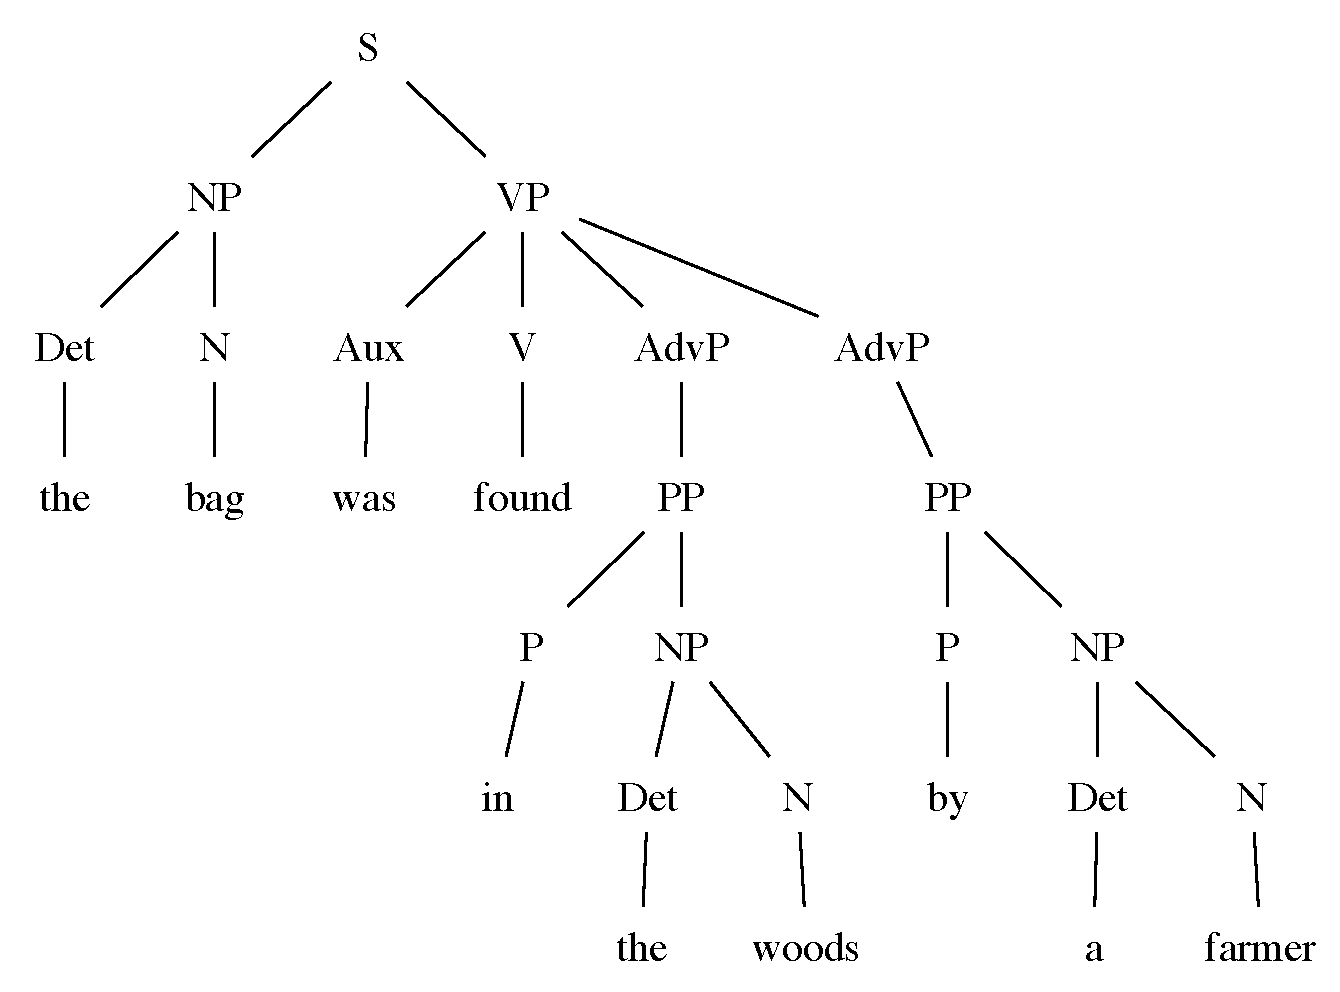
\includegraphics[scale=0.6]{ps-tree-ambig1.pdf}
\caption[One Possible Parse of \textit{the bag was found in the woods by a farmer}]{One Possible Parse of \textit{the bag was found in the woods by a farmer}, Generated from Rules in Figure~\ref{fig:ps-rules}}
\label{fig:ps-tree-ambig1}
\end{figure}
\begin{figure}[htbp]
\centering
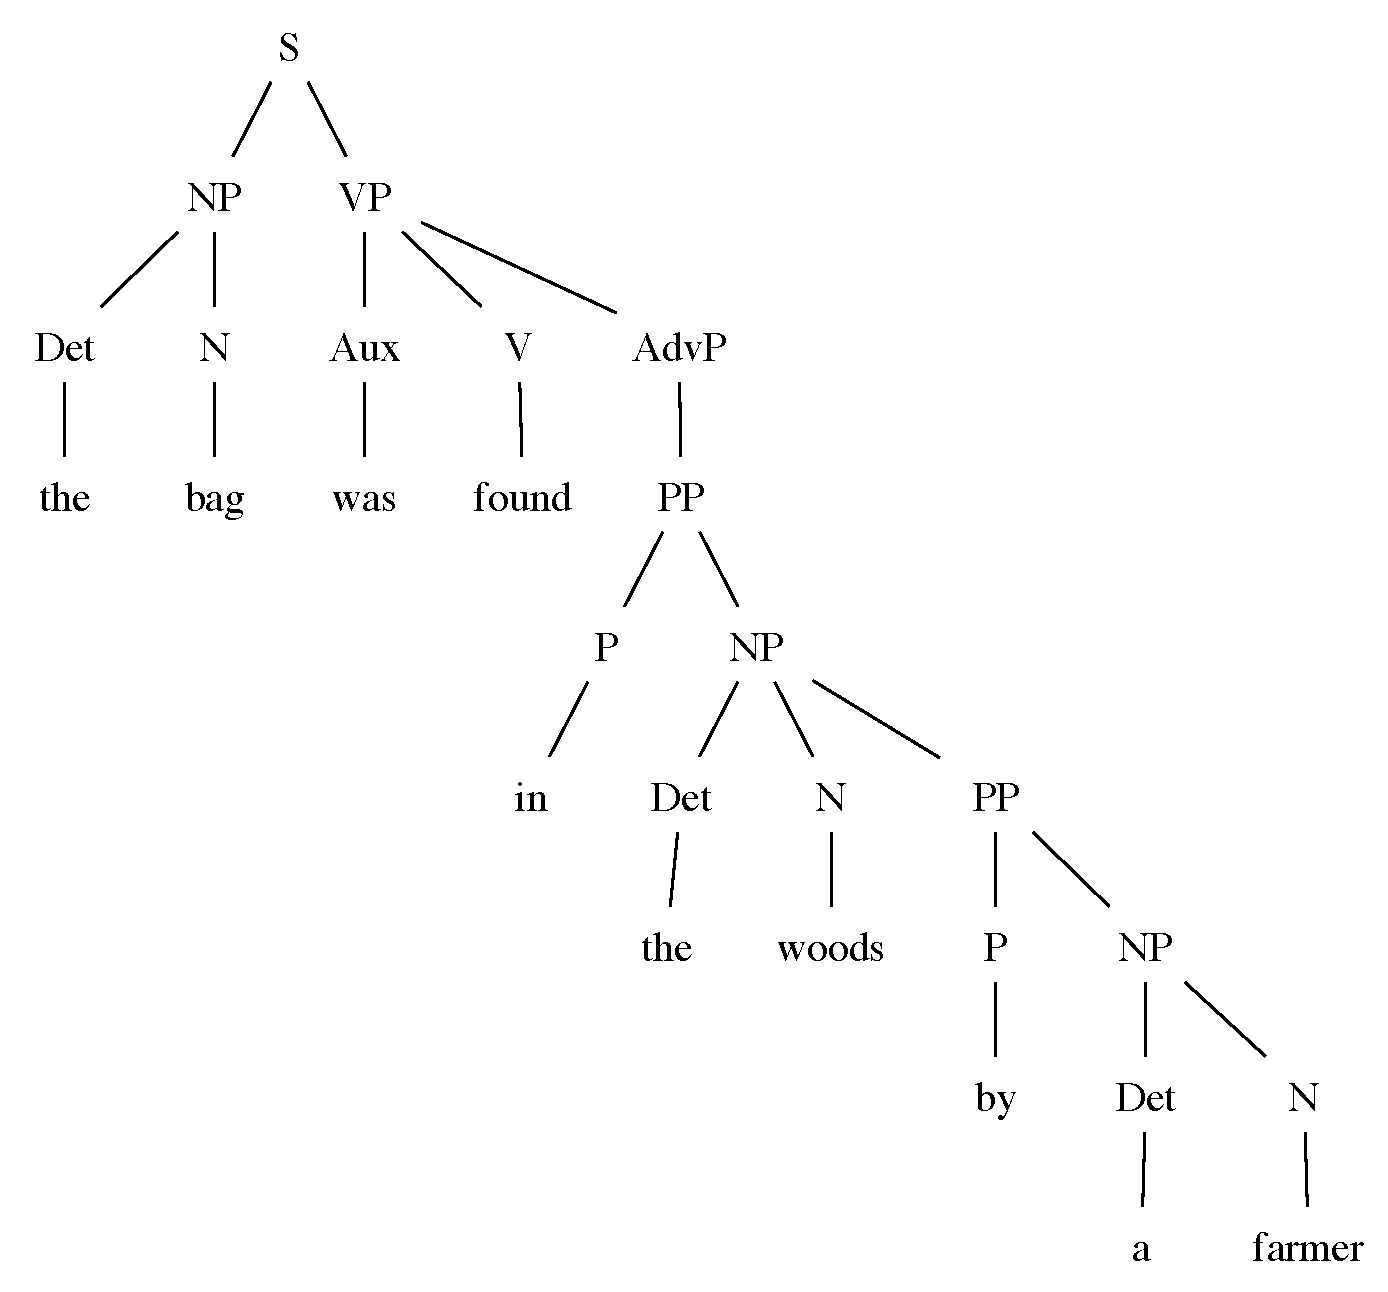
\includegraphics[scale=0.6]{ps-tree-ambig2.pdf}
\caption[Another Possible Parse of \textit{the bag was found in the woods by a farmer}]{Another Possible Parse of \textit{the bag was found in the woods by a farmer}, Generated from Rules in Figure~\ref{fig:ps-rules}}
\label{fig:ps-tree-ambig2}
\end{figure}
In both parses, the PP \textit{in the woods} is considered an adverbial phrase modifying the verb. However, the second PP can be parsed either the same way, or it can be placed within the NP containing \textit{woods}. In other words, the sentence can either mean that a farmer found the bag, or that the bag was found in the woods and those woods were located near a farmer. The first interpretation is the one that most English speakers would choose based on the semantic content of the two options. A rule-based parser, however, is unable to attempt semantic interpretation, and a purely rule-based parser might output all possible interpretations. A PCFG-based parser, however, will choose the parse that is \textit{statistically} most likely to be correct. Such a parser requires a large database of correct parses with which it can make probability measurements. The Stanford Parser, for instance, uses the Penn Treebank, a corpus of parsed English texts \citep{marcus:1993}. Out of the various possible parses, the one that a probabilistic parser will choose is the one that has a structure, or a substructure, that is most common among parses in the database. The parser does not include only the phrase structure in its consideration, but certain words as well. For instance, given \textit{the bag was found in the woods by a farmer}, the Stanford Parser will generate a parse very similar to Figure~\ref{fig:ps-tree-ambig1}. However, when given the sentence \textit{the bag was found under the bridge over the stream}, which has the same two possible parses, it chooses the other, semantically correct one. At first impression, one might think that the parser had located a semantic connection between \textit{bridge} and \textit{stream}, and had used this to choose the correct parse. However, it turns out that it is actually the prepositions (a group of closed-class words) that cause the difference in parsing. For instance, the sentence \textit{the bag was found under the woods over a farmer}, is parsed like Figure~\ref{fig:ps-tree-ambig2} and \textit{the bag was found in the bridge by the stream} is parsed like Figure~\ref{fig:ps-tree-ambig1}. Hence the parser uses both the phrase structure and the closed-class words, but generally not the open-class words, when choosing the best parse.

\subsection{The Tests}
The crux of this project was the design and creation of a suite of tests, each of which identifies a number of closely-related grammatical characteristics of the text samples. These tests operate on the output from the Stanford parser --- parse trees and grammatical dependencies. Then they generate training or test cases as output to be used by the Weka classifier. Each of these cases consists of multiple attributes, corresponding to grammatical features, each with continuous values indicating the relative frequency (probability) of that particular feature. For a case with $n$ attributes where the number of occurrences of the grammatical feature associated with the $i$th attribute is $g_i$, the value $f_i$ for that attribute is given by $g_n  / \displaystyle\sum\limits_{i=1}^n g_i$. For example, a test might measure the relative frequencies of the various tense/aspect/voice combinations of finite verbs. By one measure, English has twenty-four such combination, so the case generated by this test would have twenty-four attributes.

In addition to the attributes, each case has a class which can be \textit{es} or \textit{en}, indicating that the class is associated with a text sample written by an L1-Spanish speaker or by a native English speaker, respectively. For training cases, the classes are known beforehand and are assigned to the cases manually. For test cases, the classes have missing values until such values are determined by a classifier, as discussed in the following section.

\subsection{Classification}

The Weka machine learning package, version 3.6 \citep{hall-et-al:2009} was used to create, train and test classifiers based on the cases discussed above. Of the many classifiers included in the Weka package, two were used in this study: J48, which is Weka's implementation of the C4.5 classifier \citep{quinlan:1993} and the RandomForest classifier, which is based on the random forest algorithm described by \citet{breiman:2001}. The former is useful for its highly readable decision trees, which clearly indicate which attributes are involved in the classification and their roles. In later sections of this paper are found linguistic explanations for why these particular attributes should be useful in classification.
 
%\subsubsection{C4.5}
\addcontentsline{toc}{subsubsection}{C4.5}
\textbf{C4.5.} This section describes the C4.5 algorithm as it applies to this project. That is to say, C4.5 can deal with a number of circumstances that do not arise here. What is described here is a version of the C4.5 algorithm that is restricted to continuous attribute values and two class values, and which does not permit missing attribute values. That said, the C4.5 algorithm consists of two phases, \textit{tree construction} and \textit{tree pruning}.

In the tree construction phase a decision tree is built which successively performs binary partitioning of a set of training cases. Consider a full binary tree where each edge represents a set of cases and each non-terminal node a partitioning operation, as shown in Figure~\ref{fig:c45-dtree}. These partitioning operations take one set, represented by the parent edge, and divide it into two subsets, the daughter edges. The root node operates on an initial set $S_0$, and a leaf node simply indicates that its parent edge is a set consisting of cases of a single class. Let the first partitions of $S_0$ be called $S_1$ and $S_2$, where $S_1\cup S_2 = S_0$ and $S_1\cap S_2 = \emptyset$ , and of $S_1$ let them be called $S_{1,1}$ and $S_{2,1}$ and so forth. Likewise, let the partitioning operation that operates on a particular set be designated by $T$ with the same subscripts as that set.
\begin{figure}
\[ \xygraph{ !{<0cm,0cm>;<1cm,0cm>:<0cm,1cm>::}
!{(4,9)}*+{}="O"
!{(4,8) }*+{T_0}="t"
!{(1,7) }*+{T_1}="t1"
!{(6,7) }*+{T_2}="t2"
!{(-1,6)}*+{T_{1,1}}="t11"
!{(3,6)}*+{T_{2,1}}="t21"
!{(-2,5)}*+{C_1}="l1"
!{(-0,5)}*+{C_2}="l2"
!{(2,5)}*+{C_1}="l3"
!{(4,5)}*+{C_2}="l4"
!{(5,6)}*+{C_1}="l5"
!{(7,6)}*+{C_2}="l6"
"O":"t" _{\tiny $S_0$}
"t":"t1" _{\tiny $S_1$}
"t":"t2" ^{\tiny $S_2$}
"t1":"t11" _{\tiny $S_{1,1}$}
"t1":"t21" ^{\tiny $S_{2,1}$}
"t2":"l5" _{\tiny $S_{1,2}$}
"t2":"l6" ^{\tiny $S_{2,2}$}
"t11":"l1" _{\tiny $S_{1,1,1}$}
"t11":"l2" ^{\tiny $S_{2,1,1}$}
"t21":"l3" _{\tiny $S_{1,2,1}$}
"t21":"l4" ^{\tiny $S_{2,2,1}$}
 } \]
\caption{Decision Tree Showing the Partitioning of a Set of Training Cases $S_0$ into Subsets Consisting of Elements of a Single Class}
\label{fig:c45-dtree}
\end{figure}

Partitioning is performed by applying a binary test to each case within $S$, the set to be partitioned, and dividing the set based on the results. Each test considers a single attribute $A$ and compares the value (relative frequency) of that attribute, $V_A$, to a threshold value, $V_C$. All cases where the $V_A\leq V_C$ will be put into one subset and all other cases into the other.

The attribute and threshold value for a particular test is determined using what \citet{quinlan:1993} calls the \textit{gain ratio criterion}, which is calculated as follows. If the probability of randomly drawing a case of class $C_1$ from a set $S$ is $p_1$ and of drawing a case of the other class is $p_2$, where $p_2 = 1-p_1$, then the average amount of information needed to identify the class of a case in $S$ can be defined in terms of entropy as
\begin{equation}
\mathrm{info}(S)=-p_1 \cdot \log_2(p_1) - p_2 \cdot \log_2(p_2).
\end{equation}
A similar measure can be applied to the two partitions $S_1$ and $S_2$ created by applying the partitioning test $T$ to $S$. The entropy after partitioning is given by taking a weighted sum of the entropy of the two sets as
\begin{equation}
\mathrm{info}_T(S)=\frac{|S_1|}{|S|} \cdot \mathrm{info}(S_1) + \frac{|S_2|}{|S|} \cdot \mathrm{info}(S_2).
\end{equation}
The decrease in entropy, expressed as a positive value (an information gain), due to partitioning $S$ using the test $T$ is then
\begin{equation}
\mathrm{gain}(T)=\mathrm{info}(S)-\mathrm{info}_T(S).
\end{equation}
This gain can be used as a measurement of test fitness, with higher values indicating greater fitness, as was done in ID3, the predecessor to C4.5. However, in the more general case of C4.5, where one test can partition a set into more than 2 subsets, using this gain criterion to choose tests would favor tests that partition sets into numerous subsets. To mitigate this, Quinlan added another factor to the criterion, the \textit{split info}, which for this special case is given by
\begin{equation}
\mathrm{split\ info}(T)= -\frac{|S_1|}{|S|} \cdot \log_2 \left( \frac{|S_1|}{|S|} \right) - \frac{|S_2|}{|S|} \cdot \log_2  \left( \frac{|S_2|}{|S|}  \right).
\end{equation}
Then the fitness of a test $T$ can be measured using
\begin{equation}
\mathrm{gain\ ratio}(T) = \frac{\mathrm{gain}(T)}{\mathrm{split\ info}(T)}.
\end{equation}
It should be noted that in this special case where partitioning operations are always binary, the gain ratio criterion favors tests that split $S$ into disparately sized sets, as split info is at its maximum (unity) when $|S_1|=|S_2|$.

In choosing a test $T$, the C4.5 algorithm tries each attribute $A$ from the set $S$ of cases to be partitioned. For each, it orders the cases in $S$ on the value of $A$. If the values of $A$ corresponding to this ordered set are $\{v_1,v_2,\ldots,v_m\}$, then any threshold between some $v_i$ and $v_{i+1}$ will result in the same partitions. From this it can be seen that the total number of possible partitions is $m-1$. The algorithm tries all such partitioning schemes, measuring the gain ratio of each. When an optimal attribute and corresponding partitioning scheme has been chosen, the algorithm than chooses a threshold value that will produce this result. Again, to partition $S$ into two sets where the values for $A$ are $\{v_1,v_2,\ldots,v_i\}$ and $\{v_{i+1},v_{i+2},\ldots,v_m\}$, respectively, a threshold value $v_C$ must be chosen such that $v_i \leq v_C < v_{i+1}$. For this, it chooses the largest value for $A$ from the entire training set $S_O$ that does not exceed the midpoint of this range.

Partitioning operations are generated until a tree is produced which will divide the training set into subsets each of which contains cases of a single class. At this point a classification tree has been generated which, if fed a test case, will categorize that case into its correct class based on its attributes. In general this tree will be quite large, and, though it classifies the test cases with perfect accuracy\footnote{It is possible that the C4.5 algorithm will be unable to generate a tree that perfectly classifies the training cases. This can happen if the training set has two cases that have identical attributes and values but different classes. In this case no classifier would be able to distinguish the two.}, it will tend to be overspecialized for the test cases and will not perform as well on other cases. Both of these problems are ameliorated in the final stage, known as \textit{pruning}.

Pruning is performed by applying a statistical test to each non-terminal node to predict whether the tree would perform better in general if the subtree rooted at that node were replaced with a leaf node. To make this prediction, a certain confidence level $p$ must first be chosen, the default for C4.5 being $25\%$. Then, for any pair of numbers $N$ and $E$, where $N$ is a number of classifications and $E$ the number of those classifications which are incorrect, a value $U_{p}(E,N)$ can be calculated by taking the upper limit of the confidence interval for the binomial distribution that describes the probability of observing $E$ events in $N$ trials at a level of confidence $p$. The error of a leaf over $N$ classifications can then be estimated by computing $N\cdot U_{p}(E,N)$. The C4.5 algorithm uses this to estimate the error of a subtree by calculating this quantity for each leaf in the tree, using as $N$ the number of training cases that are classified at that node, and as $E$, the number that are classified incorrectly (generally zero), and summing these values. It then compares this estimated subtree error with the estimated error of a leaf replacing the entire subtree. In this case, $N$ will be equal to the sum of the $N$s of the leaves in the deleted subtree, and $E$ will generally be some nonzero value. If the predicted error of the leaf is less than that of the subtree, the replacement is made.

%\subsubsection{Random Forest}
\addcontentsline{toc}{subsubsection}{Random Forest}
\textbf{Random Forest.} Random forest algorithms work by using a multiple decision trees, each trained on a random subset of the training case attributes. Classification is performed by applying all decision trees to a case and choosing the most popular class, a process generally called \textit{voting}. This type of classifier was introduced by \citet{breiman:2001}, and can be generalized for use with any type of decision tree. The Weka implementation, RandomForest, uses a custom classifier for its constituent trees, the RandomTree classifier. This classifier is very similar to C4.5 without pruning, overfitting generally not being a concern with random forests \citep{breiman:2001}. The RandomForest classifier uses a customizable number of trees and attribute subset size. If the latter is not specified, the value defaults to $floor(log_2(n)+1)$ where $n$ is the number of trees. In this study, 100-tree forests were used (resulting in trees trained on 7 attributes), except when this would have resulted in an attribute subset size greater than the total number of attributes.


\biblio
\end{document}